\documentclass[svgnames,
               hyperref={colorlinks,citecolor=DeepPink4,linkcolor=FireBrick,urlcolor=Maroon},
               usepdftitle=false]  % see \hypersetup{} below
               {beamer}

\mode<presentation>{
  \usetheme{Madrid}
  \usecolortheme{seagull}
  \setbeamercovered{transparent}
  \setbeamerfont{frametitle}{size=\large}
}

\setbeamercolor*{block title}{bg=red!10}
\setbeamercolor*{block body}{bg=red!5}

%\usepackage[svgnames]{xcolor}
\usepackage{hyperref}
\hypersetup{
    pdftitle = {Making ice sheet models scale properly},
    pdfauthor = {Ed Bueler},
    pdfsubject = {},
    pdfkeywords = {}
}

\usepackage[english]{babel}
\usepackage[latin1]{inputenc}
\usepackage{times}
\usepackage[T1]{fontenc}
\usepackage{empheq,bm,xspace,fancyvrb,soul}
\usepackage{tikz}
\usetikzlibrary{shapes,arrows.meta,decorations.markings,decorations.pathreplacing,fadings,positioning}
\usepackage[kw]{pseudo}
\pseudoset{left-margin=15mm,topsep=5mm,idfont=\texttt,st-left=,st-right=}

\newcommand{\eps}{\epsilon}
\newcommand{\RR}{\mathbb{R}}

\newcommand{\grad}{\nabla}
\newcommand{\Div}{\nabla\cdot}
\newcommand{\trace}{\operatorname{tr}}

\newcommand{\hbn}{\hat{\mathbf{n}}}

\newcommand{\bb}{\mathbf{b}}
\newcommand{\be}{\mathbf{e}}
\newcommand{\bbf}{\mathbf{f}}
\newcommand{\bg}{\mathbf{g}}
\newcommand{\bn}{\mathbf{n}}
\newcommand{\bq}{\mathbf{q}}
\newcommand{\br}{\mathbf{r}}
\newcommand{\bu}{\mathbf{u}}
\newcommand{\bv}{\mathbf{v}}
\newcommand{\bw}{\mathbf{w}}
\newcommand{\bx}{\mathbf{x}}

\newcommand{\bF}{\mathbf{F}}
\newcommand{\bQ}{\mathbf{Q}}
\newcommand{\bU}{\mathbf{U}}
\newcommand{\bV}{\mathbf{V}}
\newcommand{\bX}{\mathbf{X}}

\newcommand{\btau}{\bm{\tau}}
\newcommand{\bxi}{\bm{\xi}}

\newcommand{\bzero}{\bm{0}}

\newcommand{\rhoi}{\rho_{\text{i}}}

\newcommand{\ip}[2]{\left(#1,#2\right)}

\newcommand{\mR}{R^{\bm{\oplus}}}
\newcommand{\iR}{R^{\bullet}}

\newcommand{\nn}{{\text{n}}}
\newcommand{\pp}{{\text{p}}}
\newcommand{\qq}{{\text{q}}}
\newcommand{\rr}{{\text{r}}}

\newcommand{\bus}{\bu|_s}
\newcommand{\oo}[1]{\displaystyle O\left(#1\right)}
\newcommand{\sold}{s_{\text{o}}}


\title[Making ice sheet models scale properly]{Making ice sheet models \\ scale properly}

%\subtitle{\emph{x}}

\author{Ed Bueler}

\institute[UAF]{University of Alaska Fairbanks}

\date[]{February 2023}

%\titlegraphic{\begin{picture}(0,0)
%    \put(0,180){\makebox(0,0)[rt]{\includegraphics[width=4cm]{figs/software.png}}}
%  \end{picture}
%}

\titlegraphic{\hfill 
\includegraphics[width=0.15\textwidth]{images/uafbw.png}}

%% to start section counter at 0 see
%% https://tex.stackexchange.com/questions/170222/change-the-numbering-in-beamers-table-of-content


\begin{document}
\beamertemplatenavigationsymbolsempty

%\begin{frame}
%  \maketitle
%\end{frame}

{
  \usebackgroundtemplate{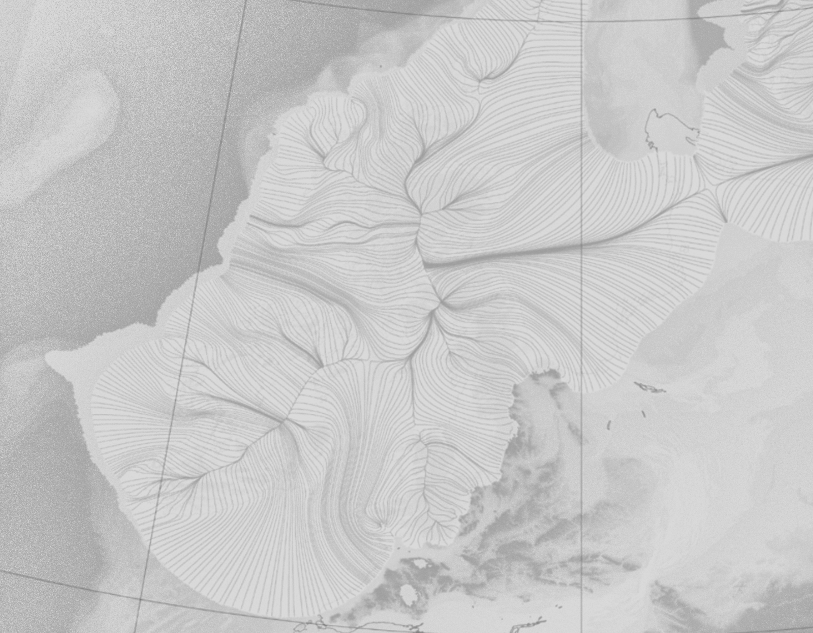
\includegraphics[width=\paperwidth]{images/gray-british-clark2022.png}}
  \begin{frame}
    \titlepage
  \end{frame}
}

\begin{frame}{Outline}
  \tableofcontents[hideallsubsections]
\end{frame}


\section{what is an ice sheet model?}

\begin{frame}{what is an ice sheet?}

\begin{itemize}
\item \emph{def.} an \alert{ice sheet} is a large glacier with small thickness$/$width
\end{itemize}

\bigskip
\begin{minipage}[t][60cm][t]{\textwidth}
\begin{center}
\includegraphics<1>[height=0.69\textheight]{images/ant-pittard2021.png}
\only<1>{\par {\scriptsize Antarctic ice sheet}} % (Pittard et al 2021)
\only<2>{\vspace{17mm}}
\includegraphics<2>[width=\textwidth]{images/ant-schoofhewitt2013.png}
\only<2>{\vspace{13mm}}
\only<2>{\par {\scriptsize note vertical exaggeration and rough bed (Schoof \& Hewitt 2013)}}
\includegraphics<3>[height=0.69\textheight]{images/alps-seguinot2018.png}
\only<3>{\par {\scriptsize modeled Alpine ice sheet near last glacial maximum (Seguinot et al 2018)}}
\includegraphics<4>[height=0.69\textheight]{images/british-clark2022.png}
\only<4>{\par {\scriptsize modeled British-Irish ice sheet near last glacial maximum (Clark et al 2022)}}
\includegraphics<5>[height=0.69\textheight]{images/not-sea-ice.png}
\only<5>{\par {\scriptsize \emph{not} sea ice!}}
\end{center}
\end{minipage}
\end{frame}


\begin{frame}{basic facts about glaciers}

\begin{columns}
\begin{column}{0.6\textwidth}
\begin{itemize}
\item glacier ice is modeled as a \emph{slow, incompressible, viscous, non-Newtonian fluid}
    \begin{itemize}
    \item[$\circ$] more on that soon
    \end{itemize}
\item glaciers lie on \emph{topography}, and sometimes they float  (\emph{ice shelf})
\item glacier geometry and velocity evolve \emph{in contact with climate}:
    \begin{itemize}
    \item[$\circ$] snowfall
    \item[$\circ$] surface melt
    \item[$\circ$] subglacial melt
    \item[$\circ$] sub-shelf melt (when floating)
    \item[$\circ$] calving (into ocean)
    \end{itemize}
\end{itemize}
\end{column}
\begin{column}{0.42\textwidth}
\hfill 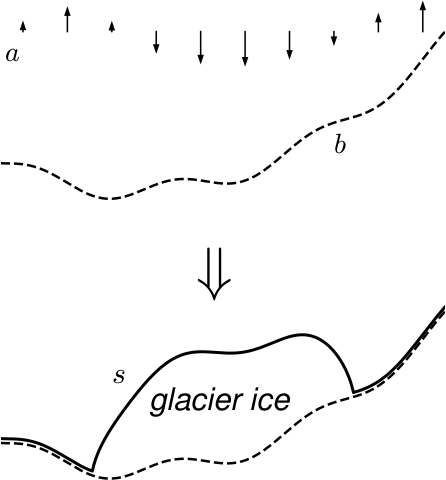
\includegraphics[width=0.9\textwidth]{images/map-glacier-ice.png}
\end{column}
\end{columns}
\end{frame}


\begin{frame}{simplifications}

\begin{columns}
\begin{column}{0.6\textwidth}
\begin{itemize}
\item for simplicity/clarity of the upcoming model performance analysis, I will ignore much of glacier physics
\item \alert{ignoring}:
    \begin{itemize}
    \item[$\circ$] floating ice
    \item[$\circ$] subglacial hydrology
    \item[$\circ$] ice temperature
    \item[$\circ$] fracture processes (calving, crevasses)
    \item[$\circ$] solid earth deformation
    \end{itemize}

\medskip
\item<2> {\footnotesize see UAF's \href{https://pism.io/}{Parallel Ice Sheet Model (\texttt{pism.io})}, for example, as a model which includes these processes}
\end{itemize}
\end{column}
\begin{column}{0.42\textwidth}
\hfill 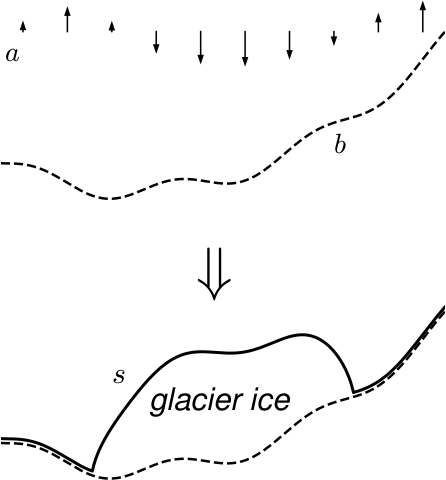
\includegraphics[width=0.9\textwidth]{images/map-glacier-ice.png}
\end{column}
\end{columns}
\end{frame}


\begin{frame}{what is an ice sheet model?}

\begin{columns}
\begin{column}{0.6\textwidth}
\begin{itemize}
\begin{definition}
an \alert{ice sheet model} is a map which simulates an ice sheet in a climate
\end{definition} 
\item at least two inputs:
    \begin{itemize}
    \item[$\circ$] \emph{surface mass balance}
$$\hspace{-7mm} a(t,x,y) = \begin{pmatrix}
\text{precipitation minus} \\
\text{melt \& runoff}
\end{pmatrix}$$

\vspace{-3mm}
        \begin{itemize}
        \item[{\scriptsize $\bullet$}] units of mass flux:\, $\text{kg}\, \text{m}^{-2} \text{s}^{-1}$
        \end{itemize}

    \item[$\circ$] \emph{bed elevation} $b(x,y)$
    \end{itemize}
\item at least two outputs:
    \begin{itemize}
    \item[$\circ$] \emph{upper surface elevation} $s(t,x,y)$
    \item[$\circ$] \emph{ice velocity} $\bu(t,x,y,z)$
    \end{itemize}

\smallskip
\item {\small \alert{map}: \, $\begin{pmatrix} \text{climate \&} \\ \text{topography} \end{pmatrix} \to \begin{pmatrix} \text{geometry} \\ \text{\& velocity} \end{pmatrix}$ }
\end{itemize}
\end{column}
\begin{column}{0.42\textwidth}
\hfill 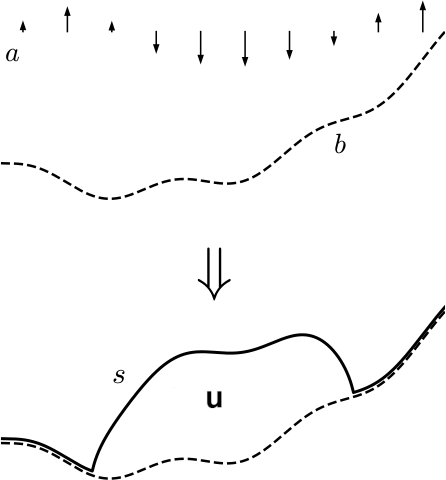
\includegraphics[width=0.9\textwidth]{images/map-velocity.png}

\vspace{2mm}
\end{column}
\end{columns}
\end{frame}


\begin{frame}{basic ice sheet model: notation}

\begin{columns}
\begin{column}{0.55\textwidth}
\begin{itemize}
\item data $a(t,x,y)$, $b(x,y)$  is defined on a \alert{fixed domain}:
	$$t \in [0,T] \quad \text{and} \quad (x,y) \in \Omega \subset \RR^2$$
\item<2-> solution surface elevation $s(t,x,y)$ is defined on $[0,T]\times \Omega$
    \begin{itemize}
    \item[$\circ$] also a fixed domain,
    \item[$\circ$] but $s=b$ where there is no ice
    \end{itemize}
\item<3> one must \emph{solve} for the time-dependent \alert{icy domain} $\Lambda(t) \subset \RR^3$, on which (solution) velocity $\bu(t,x,y,z)$ is defined:
    $$\Lambda(t) = \left\{(x,y,z)\,:\,b(x,y) < z < s(t,x,y)\right\}$$

\vspace{-2mm}
\end{itemize}
\end{column}
\begin{column}{0.46\textwidth}
\includegraphics<1>[width=\textwidth]{images/domain-data.png}

\includegraphics<2>[width=\textwidth]{images/domain-surface.png}

\includegraphics<3>[width=\textwidth]{images/domain-velocity.png}
\end{column}
\end{columns}
\end{frame}


\begin{frame}{basic ice sheet model: conservation}

\begin{itemize}
\item ice sheet evolution should conserve physical quantities:
    \begin{itemize}
    \item[$\circ$] mass
    \item[$\circ$] momentum
    \item[$\circ$] \st{energy} \hfill $\leftarrow$ \emph{ignored for simplicity in this talk}
    \end{itemize}

\medskip
\item conservation of mass is important both
    \begin{itemize}
    \item[$\circ$] in the icy domain $\Lambda(t) \subset \RR^3$:
\begin{align*}
\text{\alert{incompressibility}}&& \Div \bu &= 0 \qquad \text{in } \Lambda(t), \\
    \intertext{\item[$\circ$] and on the ice surfaces:}
\text{\alert{surface kinematic equation (SKE)}}&& \frac{\partial s}{\partial t} - \bu|_s \cdot \bn_s &= a \qquad \text{on } \Gamma_s(t), \\
\text{\alert{non-penetration}}&&     \bu|_b \cdot \bn_b &= 0 \qquad \text{on } \Gamma_b(t).
\end{align*}

        \begin{itemize}
        \item[$\vartriangleright$] $\Gamma_s(t), \Gamma_b(t) \subset \partial \Lambda(t)$ denote the surface and base of the ice
        \end{itemize}
    \end{itemize}

\end{itemize}
\end{frame}


\begin{frame}{free boundary problem}

\begin{itemize}
\item ice sheet evolution is a \alert{free-boundary} problem for conserved quantities
\item specifically, the surface kinematic equation (SKE)
  $$\frac{\partial s}{\partial t} - \bu|_s \cdot \bn_s = a$$
applies \emph{only} on the ice upper surface $\Gamma_s(t)$
\item in the remainder of the (fixed) domain $\Omega\subset \RR^2$, \alert{complementarity} holds:
  $$s=b \quad \text{and} \quad a \le 0$$

\bigskip
\item {\footnotesize for more on this perspective see Bueler (2021)}
\end{itemize}
\end{frame}


\begin{frame}{basic ice sheet model: strong form = NCP coupled to Stokes}

\begin{itemize}
\item \only<1>{\alert{nonlinear complementarity problem} (NCP)} \only<2>{nonlinear complementarity problem (NCP) coupled to \alert{Stokes}}:
\begin{align*}
s - b &\ge 0 && \text{on $\Omega \subset \RR^2$} \\
\frac{\partial s}{\partial t} - \bu|_s \cdot \bn_s - a &\ge 0 && \text{''} \\
(s - b) \left(\frac{\partial s}{\partial t} - \bu|_s \cdot \bn_s - a\right) &= 0 && \text{''} \\
\onslide<2->{- \nabla \cdot \left(2 \nu_\eps(D\bu)\, D\bu\right) + \nabla p - \rhoi \mathbf{g} &= \bzero && \text{in $\Lambda(t) \subset \RR^3$} \\
\nabla \cdot \bu &= 0 && \text{''} \\
\btau_b - \bbf(\bu|_b) &= \bzero && \text{on $\Gamma_b(t)$} \\
\bu|_b \cdot \bn_b &= 0 && \text{''} \\
\left(2 \nu_\eps(D\bu) D\bu - pI\right) \bn &= \bzero && \text{on $\Gamma_s(t)$}}
\end{align*}

    \begin{itemize}
    \item[$\circ$] $\bu|_s=0$ where no ice
    \item<2->[$\circ$] viscosity by Glen law: \, $2\nu_\eps(D\bu) = \Gamma \left(|D\bu|^2 + \eps\, D_0^2\right)^{(\pp-2)/2}$
    \end{itemize}
\end{itemize}
\end{frame}


\begin{frame}{basic ice sheet model: is a DAE system}

\begin{itemize}
\item for this slide, forget complementarity and boundary conditions
\item result: SKE coupled to Stokes
\begin{align*}
\frac{\partial s}{\partial t} - \bu|_s \cdot \bn_s - a &= 0 \\
- \nabla \cdot \left(2 \nu_\eps(D\bu)\, D\bu\right) + \nabla p - \rhoi \mathbf{g} &= \bzero \\
\nabla \cdot \bu &= 0
\end{align*}

\item only the first of these 5 equations has a time derivative
    \begin{itemize}
    \item[$\circ$] because ice is very viscous and incompressible
    \end{itemize}
\item<2> this time-dependent problem is a \alert{differential algebraic equation} (DAE), an extremely stiff system:
\begin{align*}
\dot x &= f(x,y) \\
     0 &= g(x,y)
\end{align*}

    \begin{itemize}
    \item<2>[$\circ$] but in $\infty$ dimensions (PDAE?), and subject to complementarity
    \end{itemize}
\end{itemize}
\end{frame}


\begin{frame}{basic ice sheet model: current research and thinking}

\begin{itemize}
\item to the best of my knowledge, \emph{no} current research groups are studying well-posedness or regularity for this basic model
    \begin{itemize}
    \item[$\circ$] when pressed, most researchers would agree NCP-coupled-to-Stokes is the \emph{intended} model?
    \item[$\circ$] well-posedness of the lubrication approximation of the model has been considered; existence proved in (Jouvet \& Bueler 2012)
    \end{itemize}

\medskip
\item numerical modelers tend to think of the Stokes problem separately from surface evolution
    \begin{itemize}
    \item[$\circ$] \emph{time-splitting} or \emph{explicit time-stepping} is often taken for granted
    \end{itemize}

\medskip
\item ice sheet geometry evolution is addressed with minimal awareness of complementarity

\medskip
\item NCP-coupled-to-Stokes is \emph{not yet} in common use for high-resolution, long-duration ice sheet simulations
    \begin{itemize}
    \item[$\circ$] \alert{can we make it fast enough to use?}
    \end{itemize}
\end{itemize}
\end{frame}


\AtBeginSection[]
{
  \begin{frame}{Outline}
    \tableofcontents[currentsection]
  \end{frame}
}

\section{time-stepping}

\begin{frame}{ice sheet models: the mass-continuity equation view}

\begin{itemize}
\item thickness transport form helps for evolution or stability questions
\item define:
\begin{align*}
H(t,x,y) &=s-b && \text{ice thickness} \\
\bU(t,x,y) &= \frac{1}{H} \int_b^s \bu \,dz && \begin{matrix} \text{vertically-averaged} \\ \hspace{-1.8mm} \text{horizontal velocity} \end{matrix}
\end{align*}

    \begin{itemize}
    \item[$\circ$] note $s$ and $H$ are equivalent variables for modeling ice geometry
    \end{itemize}
\item the \alert{mass continuity equation} for thickness follows from SKE and incompressibility:
   $$\frac{\partial H}{\partial t} + \nabla \cdot \left(\bU H\right) = a$$

\smallskip
\item<2> \emph{question:} is this really an advection equation?
\item<2>[] \emph{answer:} not really \dots ice flows (mostly) downhill so
  $$\bU \sim - \grad s \sim - \grad H$$
\item<2> NCP-coupled-to-Stokes DAE system has no characteristic curves
\end{itemize}
\end{frame}


\begin{frame}{mass continuity equation: advection or diffusion?}

\begin{align*}
\text{advective schema:} && \frac{\partial H}{\partial t} + \nabla \cdot \left(\bU H\right) &= a \\
\text{diffusion schema:} && \frac{\partial H}{\partial t} - \nabla \cdot \left(D \grad s\right) &= a
\end{align*}
\begin{itemize}
\item the diffusion schema is literal in the lubrication approximation
    \begin{itemize}
    \item[$\circ$] more on this momentarily
    \end{itemize}
\item but the fact that ice flows downhill has \emph{time-stepping stability} consequences
    \begin{itemize}
    \item[$\circ$] regardless of your preference for the advective schema!
    \end{itemize}
\item note both forms are highly-nonlinear: \, $\bU(H,\grad s), \, D(H,\grad s)$
\end{itemize}
\end{frame}


\begin{frame}{shallow ice approximation NCP}

\begin{itemize}
\item the simplest of several shallow approximations is the ``lubrication'' approximation, the \alert{shallow ice approximation} (SIA)
\item SIA version of the NCP:
{\small
  $$s - b \ge 0, \quad \frac{\partial s}{\partial t} + {\color{FireBrick} \Phi(s)} - a \ge 0, \quad (s - b) \left(\frac{\partial s}{\partial t} + {\color{FireBrick} \Phi(s)} - a\right) = 0$$
}
the surface motion contribution ${\color{FireBrick} \Phi(s) = - \bu|_s \cdot \bn_s}$ has a formula:
  $${\color{FireBrick} \Phi(s)} = - \frac{\gamma}{\pp} (s-b)^{\pp} |\grad s|^{\pp} - \grad \cdot\left(\frac{\gamma}{\pp+1} (s-b)^{\pp+1} |\grad s|^{\pp-2} \grad s\right)$$

\vspace{-2mm}
    \begin{itemize}
    \item[$\circ$] constants $\pp = \nn+1$ and $\gamma > 0$ relate to ice deformation
    \end{itemize}

\medskip
\item $\Phi(s)$ resolves to a \alert{doubly-nonlinear differential operator}
    \begin{itemize}
    \item[$\circ$] porous medium and $\pp$-Laplacian type simultaneously
    \item[$\circ$] \emph{local} in surface and bed topography
    \item[$\circ$] existence is known for this NCP problem (Jouvet \& Bueler, 2012), when written as a \alert{variational inequality} weak form
    \end{itemize}
\end{itemize}
\end{frame}


\begin{frame}{nonlocality}

\begin{itemize}
\item from now on, let us avoid shallowness approximations
\item then the basic ice sheet model (NCP coupled to Stokes) problem has a \alert{non-local} surface velocity function ${\color{FireBrick} \Phi(s) = - \bu|_s \cdot \bn_s}$
{\small
\begin{equation*}
s - b \ge 0, \quad \frac{\partial s}{\partial t} + {\color{FireBrick} \Phi(s)} - a \ge 0, \quad (s - b) \left(\frac{\partial s}{\partial t} + {\color{FireBrick} \Phi(s)} - a\right) = 0
\end{equation*}
}
\item \emph{figure:} the Stokes velocity solution responds to a surface perturbation by up- and down-stream changes, for several ice thicknesses, \onslide<2>{while the SIA velocity responds only underneath the surface perturbation}
\end{itemize}

\begin{center}
\includegraphics<1>[width=0.6\textwidth]{images/stokes-greens-arndt.png}
\includegraphics<2>[width=0.6\textwidth]{images/sia-greens-arndt.png}
\end{center}
\end{frame}


\begin{frame}{traditional PDE time-stepping}

{\footnotesize
\begin{align*}
\text{advective schema:} && \frac{\partial H}{\partial t} + \nabla \cdot \left(\bU H\right) &= a \\
\text{diffusion schema:} && \frac{\partial H}{\partial t} - \nabla \cdot \left(D \grad s\right) &= a
\end{align*}
}

\begin{minipage}[t][60cm][t]{\textwidth}
\begin{itemize}
\only<1>{
\item let us recall some traditional numerical analysis
}
\only<2>{
\item \alert{explicit} time stepping is common for \alert{advections}
\item for example, forward Euler using spacing $h$ and time step $\Delta t$:
	$$\frac{H_j^{\ell+1} - H_j^\ell}{\Delta t} + \frac{\bq_{j+1/2}^\ell - \bq_{j-1/2}^\ell}{h} = a_j^\ell$$

    \begin{itemize}
    \item[$\circ$] need good approximations of flux $\bq=\bU H$: upwinding, Lax-Wendroff, streamline diffusion, flux-limiters, \dots
    \item[$\circ$] conditionally stable, with CFL maximum time step
        $$\Delta t \le \frac{h}{\max |\bU|} = O(h)$$
    \end{itemize}
}
\only<3>{
\item \alert{explicit} time stepping for \alert{diffusions} is best avoided
\item for example, forward Euler:
	$$\frac{H_j^{\ell+1} - H_j^\ell}{\Delta t} - \frac{D_{j+\frac{1}{2}} (s_{j+1}^{\ell} + s_{j}^{\ell}) - D_{j-\frac{1}{2}} (s_{j}^{\ell} + s_{j-1}^{\ell})}{h^2} = a_j^\ell$$

    \begin{itemize}
    \item[$\circ$] conditionally stable, with maximum time step
        $$\Delta t \le \frac{h^2}{\max D} = O(h^2)$$
    \end{itemize}
}
\only<4>{
\item \alert{implicit} time stepping for \alert{diffusions} is often recommended
\item for example, backward Euler:
	$$\frac{H_j^{\ell+1} - H_j^\ell}{\Delta t} - \frac{D_{j+\frac{1}{2}} (s_{j+1}^{\ell+1} + s_{j}^{\ell+1}) - D_{j-\frac{1}{2}} (s_{j}^{\ell+1} + s_{j-1}^{\ell+1})}{h^2} = a_j^\ell$$

    \begin{itemize}
    \item[$\circ$] unconditionally stable, but must solve equations at each step
    \item[$\circ$] further implicit schemes: Crank-Nicolson, BDF, \dots
    \end{itemize}
}
\end{itemize}
\end{minipage}
\end{frame}


\begin{frame}{time-stepping in current and future ice sheet models}

\begin{itemize}
\item current-technology large-scale models use explicit time stepping
    \begin{itemize}
    \item[$\circ$] this is embarrassing: the mathematical problem is a DAE
    \item[$\circ$] the accuracy/performance/usability consequences of the suppressed free-boundary/DAE/diffusive character are hard to sweep under the rug
    \end{itemize}
\item most researchers believe the advection schema
    \begin{itemize}
    \item[$\circ$] time step is determined by CFL using coupled solution velocity $\bU$
    \end{itemize}

\medskip
\item \alert{implicit time-stepping} is appropriate for DAE problems
\item a sequence of NCP-coupled-to-Stokes free-boundary problems must be solved at each time step
\end{itemize}
\end{frame}


\section{stress-balance solver scaling}

\begin{frame}{the Stokes problem for ice}

\begin{itemize}
\item a non-shallow model solves a Stokes problem at each step:
\begin{align*}
- \nabla \cdot \left(2 \nu_\eps(D\bu)\, D\bu\right) + \nabla p - \rhoi \mathbf{g} &= \bzero && \text{in $\Lambda \subset \RR^3$} \\
\nabla \cdot \bu &= 0 && \text{''} \\
\btau_b - \bbf(\bu|_b) &= \bzero && \text{on $\Gamma_b$} \\
\bu|_b \cdot \bn_b &= 0 && \text{''} \\
\left(2 \nu_\eps(D\bu) D\bu - pI\right) \bn &= \bzero && \text{on $\Gamma_s$}
\end{align*}
\item this is the \alert{stress balance} (conservation of momentum) problem which determines velocity $\bu$ and pressure $p$
\item how fast is the numerical solution process?
    \begin{itemize}
    \item[$\circ$] how do solution algorithms \alert{scale} with increasing spatial resolution?
    \end{itemize}
\end{itemize}
\end{frame}


\begin{frame}{summary: PDE solver algorithmic scaling}

\begin{itemize}
\item for example, consider the 2D Poisson equation:
    $$-\grad^2 u = f \,\text{ in $\Omega$}, \qquad u=0 \,\text{ on $\partial\Omega$}$$
\item discretization generates a linear system $A\,\bu = \bb$ with $\bu\in\RR^m$
\item data size $m$ is the number of unknowns
    \begin{itemize}
    \item[$\circ$] for low-order discretizations, $m$ = \#(nodes in the grid)
    \item[$\circ$] $m$ scales with mesh cell diameter $h$: \quad $m \sim h^{-2}$ in 2D
    \end{itemize}
\item \alert{complexity} or \alert{algorithmic scaling} of flops, as $m\to\infty$, depends on solver algorithm:
    \begin{itemize}
    \item[$\circ$] $O(m^3)$ for direct linear algebra, ignoring matrix structure
    \item[$\circ$] $\approx O(m^2)$ for sparsity-exploiting direct linear algebra
    \item[$\circ$] $O(m^1)$, \alert{optimal}, e.g.~for \alert{multigrid} solvers (below)
    \end{itemize}
\end{itemize}

\medskip
\begin{center}
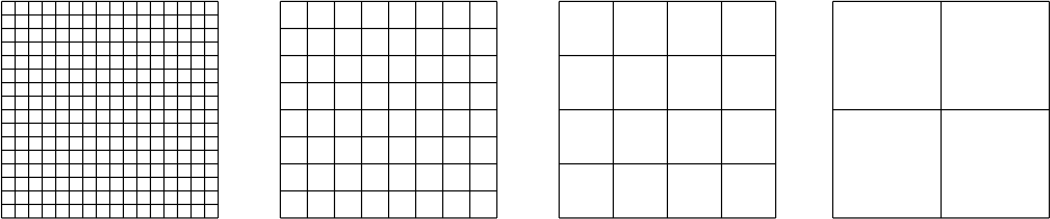
\includegraphics[width=0.5\textwidth]{images/multigrid-grids.png}
\end{center}
\end{frame}


\begin{frame}{ice sheet stress-balance solver complexity}

\begin{itemize}
\item Stokes: \quad $m$ = \#(velocity and pressure unknowns)
\item model the scaling as $O(m^{1+\alpha})$, with $\alpha=0$ optimal
\item \alert{near-optimal solvers} already exist: \hfill $\leftarrow$ \emph{good news!}
    \begin{itemize}
    \item[$\circ$] $\alpha=0.08$ for Isaac et al.~(2015) Stokes solver
        \begin{itemize}
        \item[$\vartriangleright$] unstructured quadrilateral/tetrahedral mesh, $Q_k\times Q_{k-2}$ stable elements, Schur-preconditioned Newton-Krylov, ice-column-oriented algebraic multigrid (AMG) preconditioner for $(\bu,\bu)$ block
        \end{itemize}

\begin{center}
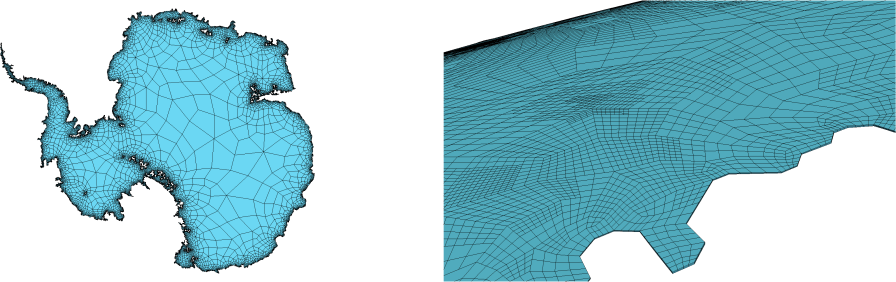
\includegraphics[width=0.6\textwidth]{images/isaac-antarctica.png}
\end{center}
    \item[$\circ$] $\alpha=0.05$ for Tuminaro et al~(2016) 1st-order (shallow) AMG solver
    \item[$\circ$] similar for Brown et al~(2013) 1st-order (shallow) GMG solver
    \end{itemize}
\end{itemize}
\end{frame}



\section{ice sheet model performance analysis}

\begin{frame}{the analysis set-up}

\begin{itemize}
\item ice sheets are thin layers, thus ice sheet models often have $O(1)$ mesh points in the vertical direction
    \begin{itemize}
    \item[$\circ$] e.g.~Issac et al (2015) Stokes solver
    \item[$\circ$] \emph{simple message}: I am ignoring refinement in the vertical
    \end{itemize}

\medskip
\item let $m$ = \#(surface elevation \& velocity \& pressure unknowns)
\item for map-plane domain $\Omega \subset \RR^2$ of width $L$ and cells of diameter $h$:
  $$m \sim \frac{L^2}{h^2} \hspace{20mm}$$

\vspace{-14mm}
\hfill
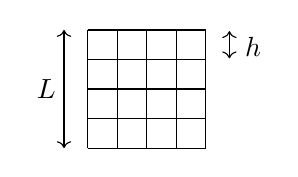
\begin{tikzpicture}[scale=1.5]
  \pgfmathsetmacro\fourth{1.0/4.0}
  \draw[xstep=\fourth,ystep=\fourth,black,thin] (0.0,0.0) grid (1.0,1.0);
  \draw[<->] (-0.2,0.0) -- (-0.2,1.0);
  \draw[<->] (1.2,0.76) -- (1.2,0.99);
  \node at (-0.35,0.5) {$L$};
  \node at (1.4,0.86) {$h$};
\end{tikzpicture}

\vspace{-2mm}
\item explicit time-stepping schemata:
{\footnotesize
\begin{align*}
\text{advective} && \frac{\partial H}{\partial t} + \nabla \cdot \left(\bU H\right) &= a & \Delta t &\le \frac{h}{U} \\
\text{diffusion} && \frac{\partial H}{\partial t} - \nabla \cdot \left(D \grad s\right) &= a & \Delta t &\le \frac{h^2}{D}
\end{align*}
}

\item stress-balance solver scaling parameterized as $O(m^{1+\alpha})$
\end{itemize}
\end{frame}


\begin{frame}{the simplified ice sheet model performance question}

\begin{itemize}
\item glaciologists want to run time-stepping high-resolution simulations of ice sheets over e.g.~$10^5$ year ice age cycles

\bigskip
\item proposed metric: \quad \alert{flops per model year}

\bigskip
\item the question:

\bigskip
\begin{center}
\begin{minipage}{0.82\textwidth}
how does this metric \alert{scale} in the \alert{high spatial resolution limit} $h\to 0$, equivalently $m\to \infty$?
\end{minipage}
\end{center}

\bigskip
\item the goal: \hspace{20mm} $O(h^{-2}) = O(m^1)$
\end{itemize}
\end{frame}


\begin{frame}{explicit ice sheet model performance}

\begin{tabular}{llll}
\emph{time-stepping} &  & \emph{flops per model year} \\ \hline
\\
explicit & SIA    & $\oo{\frac{D\, L^2}{h^{\,4}}} = \oo{\frac{D}{L^2} m^{\,2}}$ \\
\\
explicit ({\footnotesize \emph{advective}}) & Stokes \phantom{xxxx} & $\oo{\frac{U \,L^{2+2\alpha}}{h^{\,3+2\alpha}}} = \oo{\frac{U}{L} m^{1.5+\alpha}}$ \\
\\
\phantom{explicit} ({\footnotesize \emph{diffusive}})  & Stokes & $\oo{\frac{D\, L^{2+2\alpha}}{h^{\,4+2\alpha}}} = \oo{\frac{D}{L^2} m^{\,2+\alpha}}$
\end{tabular}


\vspace{10mm}
\begin{itemize}
\item explicit time-stepping implies \alert{many stress-balance solves}
    \begin{itemize}
    \item[$\circ$] while stress-balance scaling exponent $\alpha$ is important, even optimality ($\alpha=0$) cannot rescue performance
    \end{itemize}
\end{itemize}
\end{frame}


\begin{frame}{implicit time-stepping for ice sheet models}

\begin{itemize}
\item switch to \alert{implicit time-stepping} for unconditional stability?
    \begin{itemize}
    \item[$\circ$] each step is a \alert{free-boundary} NCP-coupled-to-Stokes problem
    \item[$\circ$] parameterize cost of these solves as $O(m^{1+\beta})$
    \end{itemize}
\item need $q$ model updates per year to integrate climate influences
\end{itemize}
\end{frame}


\begin{frame}{ice sheet model performance table (Bueler, 2022)}

\begin{tabular}{llll}
\emph{time-stepping} &  & \emph{flops per model year} \\ \hline
\\
explicit & SIA    & $\oo{\frac{D\, L^2}{h^{\,4}}} = \oo{\frac{D}{L^2} m^{\,2}}$ \\
\\
explicit ({\footnotesize \emph{advective}}) & Stokes \phantom{xxxx} & $\oo{\frac{U \,L^{2+2\alpha}}{h^{\,3+2\alpha}}} = \oo{\frac{U}{L} m^{1.5+\alpha}}$ \\
\\
\phantom{explicit} ({\footnotesize \emph{diffusive}})  & Stokes & $\oo{\frac{D\, L^{2+2\alpha}}{h^{\,4+2\alpha}}} = \oo{\frac{D}{L^2} m^{\,2+\alpha}}$ \\
\\
implicit & & $\oo{\frac{q\, L^{2+2\beta}}{h^{\,2+2\beta}}} = \oo{q\, m^{1+\beta}}$
\end{tabular}

\bigskip
\begin{itemize}
\item goal for optimists: implicit time-stepping \emph{and} build a $\beta \approx 0$ NCP-coupled-to-Stokes solver for the time step problems
\end{itemize}
\end{frame}


\begin{frame}{existing implicit models?}

\begin{itemize}
\item no convincing NCP-coupled-to-Stokes (free-boundary) solvers exist yet
    \begin{itemize}
    \item[$\circ$] Wirbel \& Jarosch~(2020) is an important attempt \dots
    \end{itemize}
\item the Bueler (2016) implicit (free-boundary) SIA solver scales badly: $\beta=0.8$
\end{itemize}
\end{frame}


\section{3 approaches to better performance}

\begin{frame}{approach 1: machine learning}

\begin{itemize}
\item apply \alert{machine learning}
\item run non-scalable ice sheet models on many hypothetical/real ice sheets, and train ML \alert{emulator} on results
    \begin{itemize}
    \item[$\circ$] supervised learning of physically-based model results
    \item[$\circ$] compute map on CPUs, then learn \& evaluate map on GPUs
    \item[$\circ$] convincing demo in Jouvet et al.~(2021)
    \end{itemize}
\end{itemize}

\vspace{3mm}
\begin{minipage}[t][60cm][t]{\textwidth}
\begin{center}
\only<1>{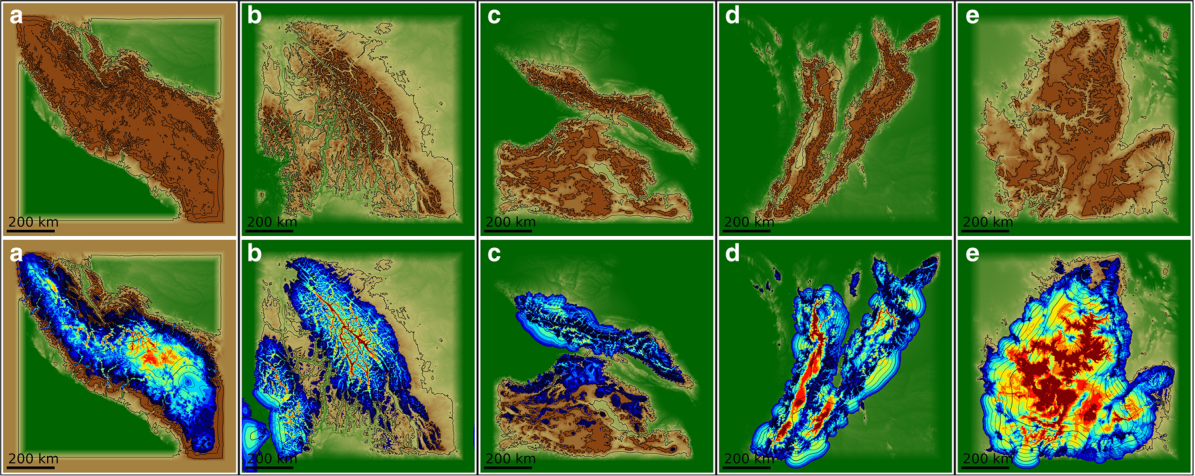
\includegraphics[height=0.52\textheight]{images/tiles-jouvet.png}}
\only<2>{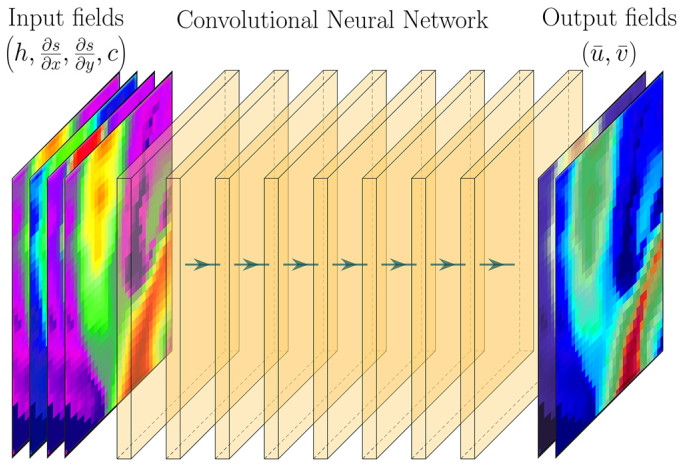
\includegraphics[height=0.57\textheight]{images/cnn-jouvet.png}}
\end{center}
\end{minipage}
\end{frame}


\begin{frame}{approach 2: semi-coupled time-stepping}

\begin{itemize}
\item idea from L{\"o}fgren et al.~(2022)
    \begin{itemize}
    \item[$\circ$] earlier use in mantle/crust simulations (Kaus et al.~2010)
    \end{itemize}
\item \emph{idea.} remain explicit, but \alert{modify the Stokes problem to ``see'' the updated (extrapolated) surface}
\item that is, modify the Stokes problem at time $t^\ell$ \onslide<2>{by adding body force terms corresponding to the updated-surface icy domain}

\vspace{-3mm}
\begin{minipage}[t][30mm][t]{0.8\textwidth}
\only<1>{
{\small
\begin{align*}
\int_{\Lambda^\ell} 2 \nu D\bu : D\bv - \int_{\Lambda^\ell} p \Div \bv &= \int_{\Lambda^\ell} \bbf\cdot \bv \\
\phantom{x} \\
\phantom{x} \\
\int_{\Lambda^\ell} q \Div \bu &= 0
\end{align*}
}
}
\only<2>{
{\small
\begin{align*}
\int_{\Lambda^\ell} 2 \nu D\bu : D\bv - \int_{\Lambda^\ell} p \Div \bv \qquad\qquad &= \int_{\Lambda^\ell} \bbf\cdot \bv + \Delta t \int_{\Gamma_s^\ell} a\, (\bbf\cdot \bv)\,dx\\
\hspace{20mm} - \Delta t \int_{\Gamma_s^\ell} (\bu \cdot \bn_{s^\ell}) (\bbf\cdot \bv)\,dx \qquad
&\phantom{=} \\
\int_{\Lambda^\ell} q \Div \bu &= 0
\end{align*}
}
}
\end{minipage}

\bigskip
\item<2> early experiments suggest $\sim 10$ times longer stable time steps
\end{itemize}

\end{frame}


\begin{frame}{approach 3: multilevel NCP-coupled-to-Stokes solvers}

\begin{itemize}
\item direct attack on the problem seems to require a \alert{multilevel} solver for \alert{variational inequalities} (VIs)
\item but in the \alert{non-local residual case} \hfill $\gets$ \emph{yesterday's seminar}
    \begin{itemize}
    \item[$\circ$] this seems not to exist
    \item[$\circ$] the \alert{smoother} must reduce a residual formed from surface-motion term $\Phi(s) = - \bu|_s\cdot \bn_s$ (from a scalable Stokes solver)
    \end{itemize}
\item near-optimal multilevel solvers exist for simpler VI problems
\end{itemize}
\end{frame}


\section{conclusion}

\begin{frame}{\alert{summary}}

\begin{itemize}
\item ice sheet models solve a multi-scale, irregular-data problem with hard-to-observe boundary conditions
   \begin{itemize}
   \item[$\circ$] there are \alert{no easy or magic techniques} for performance
   \end{itemize}
\item<2-> current-technology ice sheet models mostly use \alert{explicit} time stepping, \alert{non-optimal} stress-balance solvers, and \alert{shallow} assumptions
   \begin{itemize}
   \item[$\circ$] progress is being made in all of these areas
   \end{itemize}
\item<3-> \alert{coming soon} from current research:
   \begin{enumerate}
   \item[1.] machine learning emulators (Jouvet et al.~2021)
   \item[2.] semi-coupled time stepping (L{\"o}fgren et al.~2022)
   \item[3.] scalable Stokes solvers (Isaac et al.~2015)   
   \end{enumerate}
\item<4-> scalable solvers for implicit-step NCP-coupled-to-Stokes models, which would seem to be the recommended numerical design, require \alert{multilevel solvers for non-local variational inequalities}
\end{itemize}
\end{frame}


\begin{frame}{references}

{\scriptsize
\begin{itemize}
\item E.~Bueler (2016). \emph{Stable finite volume element schemes for the shallow-ice approximation}, J.~Glaciol.~62 (232), 230--242, \href{https://doi.org/10.1017/jog.2015.3}{10.1017/jog.2015.3}
\item E.~Bueler (2021). \emph{Conservation laws for free-boundary fluid layers}, SIAM J.~Appl.~Math.~81 (5), 2007--2032, \href{https://doi.org/10.1137/20M135217X}{10.1137/20M135217X}
\item E.~Bueler (2022). \emph{Performance analysis of high-resolution ice-sheet simulations}, J.~Glaciol., \href{https://doi.org/10.1017/jog.2022.113}{10.1017/jog.2022.113}
\item T.~Isaac, G.~Stadler, \& O.~Ghattas (2015). \emph{Solution of nonlinear Stokes equations discretized by high-order finite elements on nonconforming and anisotropic meshes, with application to ice sheet dynamics}, SIAM J.~Sci.~Comput.~37 (6), B804--B833, \href{https://doi.org/10.1137/140974407}{10.1137/140974407}
\item G.~Jouvet \& E. Bueler (2012). \emph{Steady, shallow ice sheets as obstacle problems: well-posedness and finite element approximation}, SIAM J.~Appl.~Math. 72 (4), 1292--1314, \href{https://doi.org/10.1137/110856654}{10.1137/110856654}
\item G.~Jouvet, G.~Cordonnier, B.~Kim, M.~L\"uthi, A.~Vieli, A.~Aschwanden (2021). \emph{Deep learning speeds up ice flow modelling by several orders of magnitude}, J.~Glaciol.~\href{https://doi.org/10.1017/jog.2021.120}{10.1017/jog.2021.120}
\item A.~L{\"o}fgren, J. Ahlkrona, \& C. Helanow (2022). \emph{Increasing stable time-step sizes of the free-surface problem arising in ice-sheet simulations}, J.~Comput.~Phys.~X 16, \href{https://doi.org/10.1016/j.jcpx.2022.100114}{10.1016/j.jcpx.2022.100114}
\end{itemize}
}
\end{frame}

\end{document}
